\section{Results}
\label{sec:results}

\subsection{Metrics for Order Bias}
\label{sec:metrics}

To quantify the impact of answer permutation on model predictions, we adopt three metrics widely used in recent work: \textbf{Relative Standard Deviation (RSD)} \citep{reif-schwartz-2024-beyond}, \textbf{Recall Standard Deviation (RStd)} \citep{zheng2024largelanguagemodelsrobust}, and \textbf{Fluctuation Rate (FR)} \citep{wei-etal-2024-unveiling}.  
Each captures a different facet of instability under order variation.

\paragraph{Relative Standard Deviation (RSD).}
RSD measures the sensitivity of overall accuracy to answer permutations.  
Let $\{A_1,A_2,\dots,A_n\}$ denote the model’s accuracy under $n$ distinct answer orders. Then
\begin{align}
  \mathrm{RSD} &=
  \frac{\sqrt{\frac{1}{n}\sum_{i=1}^{n}(A_i-\overline{A})^2}}
       {\overline{A}}, \\
  \overline{A} &= \frac{1}{n}\sum_{i=1}^{n}A_i .
  \label{eq:rsd}
\end{align}
Higher values indicate greater variability in model-level performance across permutations.

\paragraph{Recall Standard Deviation (RStd).}
RStd captures how individual questions are affected by order shifts.  
For each question $q$, let $\{r_{q,1},\dots,r_{q,k}\}$ be the binary correctness across $k$ permutations. Then
\begin{align}
  \mathrm{RStd} &=
  \frac{1}{N}\sum_{q=1}^{N}
  \frac{
    \sqrt{\frac{1}{k}\sum_{j=1}^{k}(r_{q,j}-\overline{r_q})^2}
  }{
    \overline{r_q}+\varepsilon
  }, \\
  \overline{r_q} &= \frac{1}{k}\sum_{j=1}^{k}r_{q,j}.
  \label{eq:rstd}
\end{align}
Here $\varepsilon$ is a small constant to prevent division by zero. A larger RStd signals greater sample-level prediction instability.

\paragraph{Fluctuation Rate (FR).}
FR quantifies how often the predicted answer changes when the option order is permuted.  
Let $f_q$ be the number of unique predictions for question $q$ across the $k$ permutations:
\begin{equation}
  \mathrm{FR}=
  \frac{1}{N}\sum_{q=1}^{N}\frac{f_q-1}{k-1}.
  \label{eq:fr}
\end{equation}
FR ranges from $0$ (fully stable) to $1$ (changes prediction in every permutation), directly reflecting positional sensitivity.

\subsection{Overall Results}

The overall performance of each method across English and Chinese datasets are summarized in Table~\ref{tab:order_bias_results}, and Figure~\ref{fig:overall_results} visualizes the results of each method across metrics. Our proposed CA-adjusted MCQ Answering method (specifically with cutoff value 0.2) consistently reduced order bias compared to both Direct Prompting and CoT prompting across all evaluated metrics, only being beaten in RSD by the SoTA Direct Prompting method.

\begin{figure}[t]
    \centering
    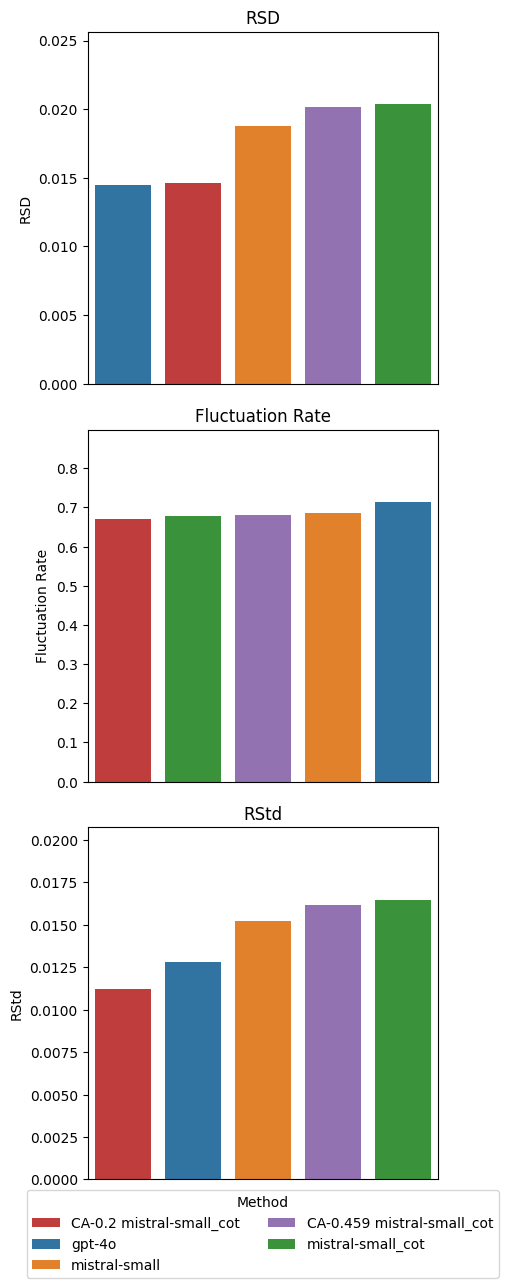
\includegraphics[height=0.63\textheight]{figures/overall.png}
    \caption{Comparison of the five methods on RSD, RStd, and Fluctuation Rate. Lower values indicate reduced order bias and improved stability.}
    \label{fig:overall_results}
\end{figure}

\begin{table*}[t]
\centering
\resizebox{\textwidth}{!}{
\begin{tabular}{l|cc|cc|cc|cc|}
\cline{2-9}
 & \multicolumn{2}{c|}{\textbf{Overall Accuracy}} & \multicolumn{2}{c|}{\textbf{RSD}} & \multicolumn{2}{c|}{\textbf{RStd}} & \multicolumn{2}{c|}{\textbf{Fluctuation Rate}} \\
\hline
\multicolumn{1}{|l|}{\textbf{Method}} & \textbf{English} & \textbf{Chinese} & \textbf{English} & \textbf{Chinese} & \textbf{English} & \textbf{Chinese} & \textbf{English} & \textbf{Chinese} \\
\hline
\multicolumn{1}{|l|}{\textbf{gpt-4o}} & \textbf{0.882794} & \textbf{0.849265} & \textbf{0.014487} & \textbf{0.019291} & 0.012789 & \textbf{0.016383} & 0.713088 & 0.701176 \\
\multicolumn{1}{|l|}{\textbf{mistral-small}} & 0.810441 & 0.733333 & 0.018762 & 0.032797 & 0.015205 & 0.024051 & 0.686029 & 0.658500 \\
\multicolumn{1}{|l|}{\textbf{mistral-small\_cot}} & 0.809412 & 0.748676 & 0.020342 & 0.044451 & 0.016465 & 0.033279 & 0.679265 & 0.660735 \\
\multicolumn{1}{|l|}{\textbf{CA-0.2 mistral-small\_cot}} & 0.766618 & 0.698235 & 0.014643 & 0.032861 & \textbf{0.011226} & 0.022945 & \textbf{0.671176} & \textbf{0.654412} \\
\multicolumn{1}{|l|}{\textbf{CA-0.459 mistral-small\_cot}} & 0.804118 & 0.743824 & 0.020140 & 0.042449 & 0.016195 & 0.031575 & 0.679559 & 0.660147 \\
\hline
\end{tabular}}
\caption{Evaluation of models across English and Mandarin on Overall Accuracy, Relative Standard Deviation (RSD), Recall Standard Deviation (RStd), and Fluctuation Rate (FR). For RSD, RStd, and FR lower scores indicate less order bias}
\label{tab:order_bias_results}
\end{table*}




\subsection{Order Sensitivity Across Languages}

We conducted our experiment with both English and Chinese to compare the order bias between the two languages. RSD, RStd, and Fluctuation Rate all varied by language across methods (see Figure~\ref{fig:language_results}), with RSD and RStd being consistently higher in Chinese than English, and Fluctuation Rate consistently being slightly lower.

Observing RSD and RStd across methods, our SoTA Direct Prompting method exceeds our CA-Adjusted method. This is likely a result of better multilingual capabilities in our SoTA GPT-4o model as opposed to mistral-small. The full results across languages can be found in Table~\ref{tab:order_bias_results}

\begin{figure*}[t]
    \centering
    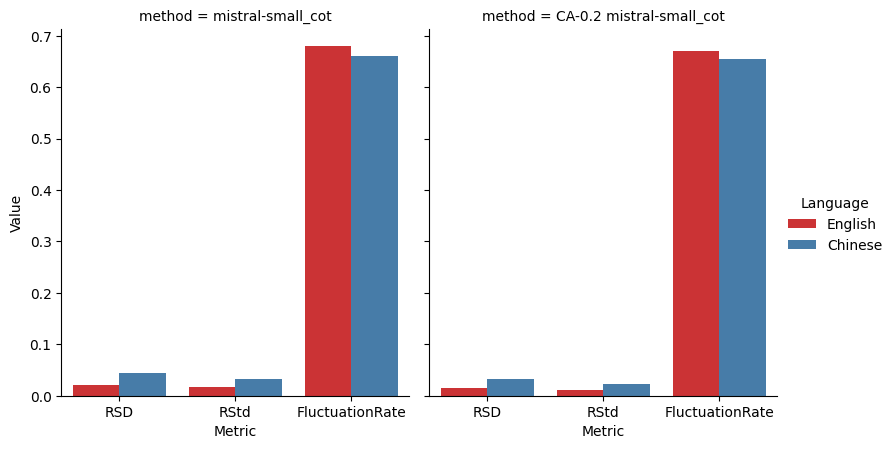
\includegraphics[width=\textwidth]{figures/language.png}
    \caption{Comparison of English vs. Mandarin for RSD, RStd, and Fluctuation Rate across \texttt{mistral-small\_cot} and \texttt{CA-0.2 mistral-small\_cot} methods. Lower RSD, RStd, or Fluctuation Rate values indicate reduced order bias}
    \label{fig:language_results}
\end{figure*}

\subsection{Order Sensitivity Across Subcategories}

To observe order bias in different knowledge domains, we contrast our metrics across the 17 subcategories defined in \citet{hendryckstest2021}, comparing SoTA Direct Prompting, CoT, and CA-adjusted CoT (with cutoff value 0.2 results). Figure~\ref{fig:subcategory_rsd} illustrates the English RSD values by subcategory for \texttt{mistral-small\_cot} versus \texttt{CA-0.2 mistral-small\_cot}.

Across these subcategories, the CA-Adjusted MCQ Answering method achieved lower values on a majority of metrics, improving order bias in 14 out of 17 cases. The subcategories in which CA-adjustment did not improve order bias include computer science, economics, and psychology. The full results across subcategories are found in Table~\ref{tab:order_bias_results}


\begin{figure*}[t]
    \centering
    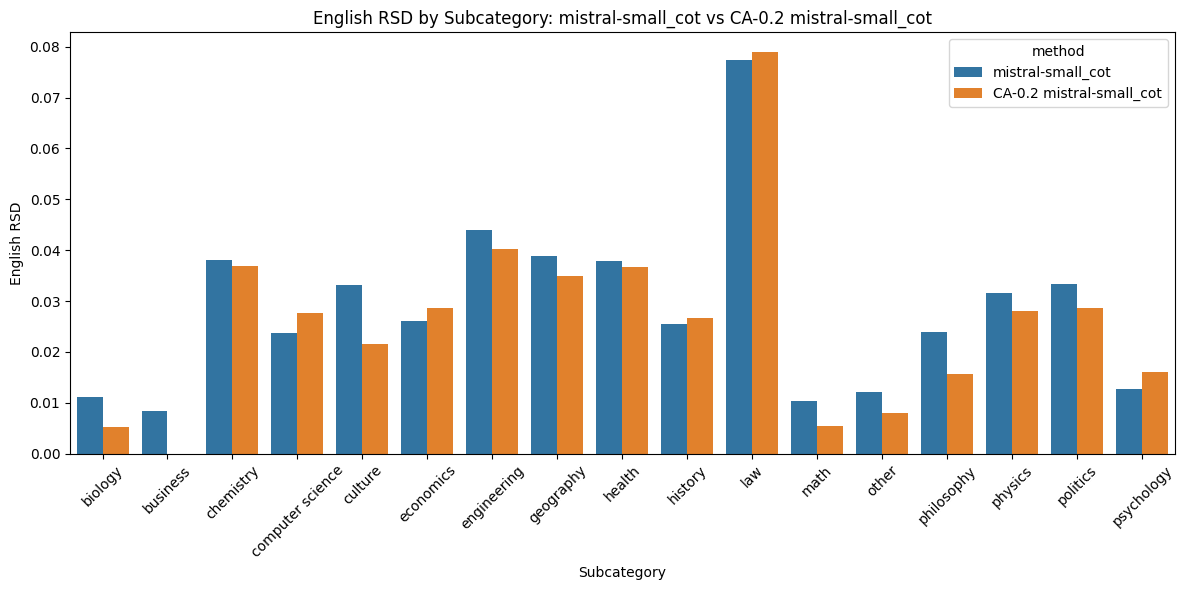
\includegraphics[width=\textwidth]{figures/subcategory.png}
    \caption{English RSD by Subcategory comparing \texttt{mistral-small\_cot} (blue) vs. \texttt{CA-0.2 mistral-small\_cot} (orange). Orange bars higher than blue indicate subcategories in which CA-Adjustment reduced order bias.}
    \label{fig:subcategory_rsd}
\end{figure*}


\subsection{Confidence vs. Order Bias}

Our CA-Adjusted method allows us to control the balance between order-bias reduction and accuracy by adjusting the cutoff value. A higher cutoff value results in less answer choices being removed, retaining accuracy but having little to no effect on order bias. A lower cutoff value removes more answer choices, lowering order bias more, but decreases accuracy as the chances of the correct answer being accidentally removed rise.

In our experiment, CA-Adjusted with cutoff value 0.2 clearly outperformed 0.459 in all recorded metrics as shown in Figure~\ref{fig:overall_results}, while cutoff value 0.459 was outperformed by Direct Prompting in both RStd and Fluctuation Rate. That being said, Table~\ref{tab:accuracy_results} shows the decreased accuracy of a cutoff value of 0.459 as opposed to 0.2. CA-Adjusted with a 0.459 cutoff value performs 5.04\% and 7.09\% better than with 0.2 in English and Chinese respectively.

Although the results of this test specifically compared the two cutoff values of 0.2 and 0.459, future research might benefit from exploring the impacts of further tuning of the cutoff value, as well as alternate ways of determining extraneous answer choices based on similarity scores.

\subsection{Takeaways from Cognitive Alignment} %maybe change the name
\label{sec:takeaways}

Cognitive Alignment and CA-Adjusted MCQ Answering both were successful in lowering order bias across knowledge domains and languages.

However, we also found a number of obvious drawbacks of the CA approach. For example, in the following question/answer pair we see a complete failure based on the format of the question:

\noindent\textbf{Question} \\
What was 'democratic enlargement'?

\vspace{0.5em}

\noindent\textbf{Answer choices}
\begin{enumerate}[label=\Alph*., itemsep=0pt, topsep=0pt]
    \item A proposal for reform of the US system of government
    \item A proposal for the extension of democratic rule globally
    \item A proposal for the extension of free markets
    \item Both b and c
\end{enumerate}


\vspace{0.5em}

\noindent\textbf{Free-response answer generated by CA method:} \\
\textit{Democratic enlargement refers to the process of expanding democratic governance and institutions, often within a region or globally. It involves promoting democracy in countries that are transitioning from authoritarian regimes or have limited democratic practices. This can include efforts such as supporting free elections, strengthening civil society, and fostering human rights.}

\vspace{0.5em}

\noindent\textbf{Similarity scores generated by CA method}

\begin{center}
\begin{tabular}{@{}ll@{}}
\toprule
\textbf{Choice} & \textbf{Similarity Score} \\
\midrule
A & 0.1847597062587738 \\
B & 0.517923891544342 \\
C & 0.19801126420497894 \\
D & -0.06396911293268204 \\
\bottomrule
\end{tabular}
\end{center}

While "Both b and c" is the correct answer, the alignment method cannot detect the similarity between it and the free response answer because the answer choice merely references other answer choices. 

Overall, it is clear that this method produces a tradeoff between accuracy and reduced order bias. Our most successful method at reducing order bias, CA-0.2 mistral-small\_cot, led to a 5.49\% and 7.57\% accuracy decrease in English and Chinese respectively. A full comparison of accuracy across CA methods is located in Table~\ref{tab:accuracy_results}.



\begin{table}[h]
\centering
\small
\begin{tabular}{|l|c|c|}
\hline
\textbf{Method} & \textbf{English} & \textbf{Chinese} \\
\hline
Pure CA & 0.43000 & 0.38353 \\
CA-0.2 mistral-small\_cot & 0.77059 & 0.69706 \\
CA-0.459 mistral-small\_cot & 0.80941 & 0.74647 \\
mistral-small\_cot & 0.81529 & 0.75412 \\
\hline
\end{tabular}
\caption{Accuracy of each method on English and Chinese.}
\label{tab:accuracy_results}
\end{table}


\subsection{Future Research Paths} %maybe don't make a subsection
While the lackluster accuracy performance of the pure CA method would suggest it shouldn't be used in multiple choice answering as is, the inherent, complete removal of order bias suggests incorporating alignment might still be useful in reducing order bias. 

The CA-Adjusted method provides an example of how this could be done, but falls short of a widely implementable method. Future research might refine the method of deciding on specific answer choices to remove to avoid issues like those shown in~\ref{sec:takeaways}, or use other methods of removing problematic answer choices before being feeding the ordered questions to an LLM.

The code and experimental framework used in this paper are available at: \url{https://github.com/softly-undefined/NLP_final}.
